\documentclass[a4paper,12pt]{report} %%%{article}

\usepackage{cmap} % searchable PDFs
\usepackage[T2A]{fontenc} % scalable fonts
\usepackage[utf8]{inputenc} % input in UTF8
\usepackage[english,russian]{babel} % dashes on linebreaks
\usepackage{indentfirst} % indents in paragraphs
\usepackage{amstext,amssymb,amsfonts,amsmath,mathtext,enumerate,float}
\usepackage[left=25mm,right=2cm,top=2cm,bottom=2cm,bindingoffset=0cm]{geometry}
\usepackage[unicode]{hyperref}
\usepackage{graphicx}
\usepackage{ulem} % strikethrough
\usepackage{verbatim} % multiline comments
\usepackage{hhline}

\usepackage{listings}
\usepackage{color}
 
\lstset{extendedchars=\true}
  
\definecolor{dkgreen}{rgb}{0,0.6,0}
\definecolor{gray}{rgb}{0.5,0.5,0.5}
\definecolor{mauve}{rgb}{0.58,0,0.82}
 
\lstset{ %
  columns=flexible,
%  language=C,                     % the language of the code
  basicstyle=\footnotesize\ttfamily,       % the size of the fonts that are used for the code
  numbers=left,                   % where to put the line-numbers
  numberstyle=\tiny\color{gray},  % the style that is used for the line-numbers
  stepnumber=1,                   % the step between two line-numbers. If it's 1, each line will be numbered
  numbersep=5pt,                  % how far the line-numbers are from the code
  backgroundcolor=\color{white},  % choose the background color. You must add \usepackage{color}
  showspaces=false,               % show spaces adding particular underscores
  showstringspaces=false,         % underline spaces within strings
  showtabs=false,                 % show tabs within strings adding particular underscores
%  frame=single,                   % adds a frame around the code
  rulecolor=\color{black},        % if not set, the frame-color may be changed on line-breaks within not-black text (e.g. comments (green here))
  tabsize=4,                      % sets default tabsize
  captionpos=b,                   % sets the caption-position to bottom
  breaklines=true,                % sets automatic line breaking
  breakatwhitespace=false,        % sets if automatic breaks should only happen at whitespace
  title=\lstname,                 % show the filename of files included with \lstinputlisting; also try caption instead of title
  keywordstyle=\color{blue},      % keyword style
  commentstyle=\color{dkgreen},   % comment style
  stringstyle=\color{mauve},      % string literal style
%  escapeinside={\%*}{*)},         % if you want to add LaTeX within your code
  mathescape=true,
  morekeywords={*,...},           % if you want to add more keywords to the set
  deletekeywords={...},           % if you want to delete keywords from the given language
  aboveskip=1em,
  belowskip=-1em
}


\usepackage{mathtools}
\newcommand{\defeq}{\vcentcolon=}
\newcommand{\eqdef}{=\vcentcolon}

\renewcommand{\contentsname}{Содержание} 
\setcounter{secnumdepth}{0}
\setcounter{tocdepth}{3}

% \linespread{1.3}
\sloppy % align=justify


% \title{Схема сборки проекта с~агрессивным переиспользованием порождений}
	   
\author[Сергей Серебряков]{Сергей Серебряков}

\institute[СПбГУ]{
	\textbf{кафедра системного программирования}\\ 
	\textbf{математико-механический ф-т, СПбГУ}\\
	\texttt{sergey@serebryakov.info}
}

\date{
	\textbf{СПИСОК-2013}
}
\title{Схема сборки проектов с~агрессивным переиспользованием порождений}
% \title[{\makebox[.45\paperwidth]{\hfill\insertframenumber/\inserttotalframenumber}}]{
% 	Схема сборки проектов с~агрессивным переиспользованием порождений
% }

\author[Сергей Серебряков]{
  \text{Сергей Серебряков, 545 группа}\\
}

\institute[]{
  \begin{tabular}[h]{rl}
      Научный руководитель: &к.ф.-м.н.~Д.~Ю.~Булычев \\
      Рецензент: &к.ф.-м.н.~Н.~В.~Чашников
  \end{tabular}      
}

\date{28 мая 2013}


\begin{document}

{
	\setbeamertemplate{footline}{}
	\begin{frame}
		\titlepage
	\end{frame}
}
\addtocounter{framenumber}{-1}

\begin{frame}{Введение}
\begin{itemize}
	\item Сборка программного проекта
	\item Инкрементальная компиляция
	\item Кэш компиляции
	\item Переиспользование кэшей в большом проекте
\end{itemize}
\begin{figure}[!h]
	\begin{center}
		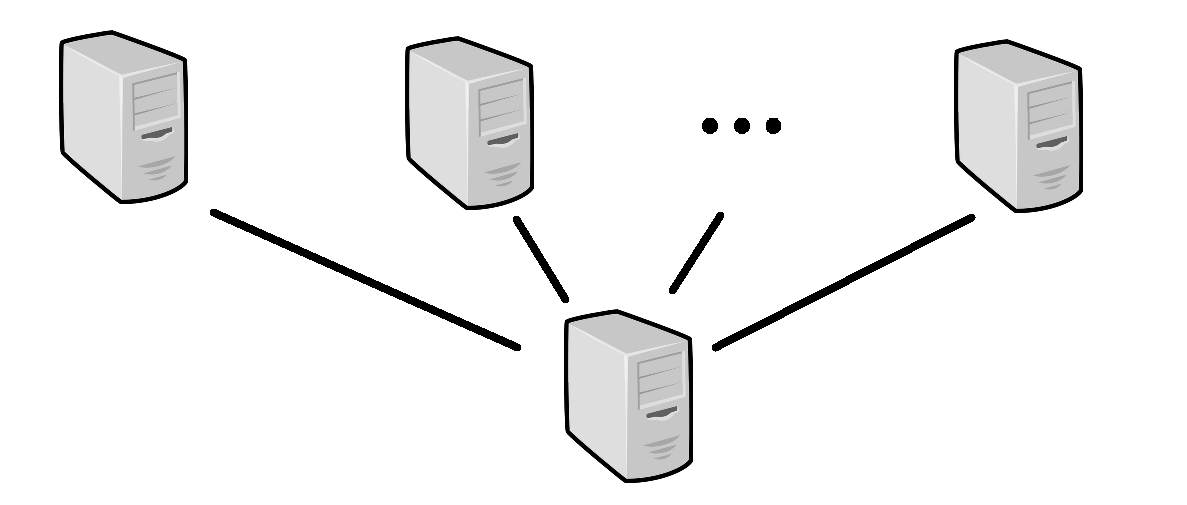
\includegraphics[width=80mm]{network.png}
	\end{center}
\end{figure}
\end{frame}

\begin{frame}{Постановка задачи}
\begin{itemize}
	\item Построить формальную модель предметной области
	\item Сформулировать в терминах этой модели и решить задачу инкрементальной компиляции и задачу переиспользования порождений
\end{itemize}
\end{frame}

\begin{frame}{Основные определения}

$\Sigma$ --- множество входов, $\Omega$ --- множество выходов\\
Функция порождения выходов по входам (частичная):
$$gen : 2^\Omega \times 2^\Sigma \to 2^\Omega$$

\end{frame}

\begin{frame}{Аксиомы}
\begin{enumerate}
	\item Аксиома о переопределённости: если $gen(\omega,\sigma)$~--- определена, то $\omega\cap gen(\omega,\sigma) = \varnothing$
	
	\item Аксиома о дизъюнктном разбиении: если $gen(\omega,\sigma) = \omega^\prime$, то существует единственное дизъюнктное разбиение $\omega^\prime=\bigcup^\varnothing_{s\in\sigma}\omega^\prime_s$, 
	удовлетворяющее свойству 

	$$\forall s\in\sigma : gen(\omega\cup\omega^\prime\setminus\omega^\prime_s,\{s\})=\omega^\prime_s$$
\end{enumerate}
\end{frame}

\begin{frame}{Аксиомы}
\begin{enumerate}
	\setcounter{enumi}{2}
	\item Аксиома об эквивалентных контекстах: $\forall s\in\Sigma,\; \forall\omega,\:\omega^\prime\subseteq\Omega:$ если $s$ невырожденное, $gen(\omega,\{s\})$ определено и $B^0_{\omega} = B^0_{\omega^\prime}$, то и $gen(\omega^\prime,\{s\})$ определено, более того, $gen(\omega,\{s\}) = gen(\omega^\prime,\{s\})$

	\item Аксиома о минимально необходимом контексте: если $gen(\omega,\{s\})$~--- определена, то в $\omega$ существует наименьшее по включению подмножество $d_\omega(s)$, такое, что $gen(d_\omega(s), \{s\})$~--- определена
\end{enumerate}
\end{frame}

\begin{frame}{Аксиомы}
\begin{enumerate}
	\setcounter{enumi}{4}
	\item Аксиома о недоопределённости: если $gen(\omega, \sigma) = \omega^\prime$ и для какого-то $s\in\sigma$ существует $s_1\in\sigma$, такой, что $d_{\omega\cup\omega^\prime\setminus\omega^\prime_s}(s) \cap \omega^\prime_{s_1}\ne\varnothing$, то $gen(\omega, \sigma\setminus s_1)$ не определена
	
	\item Аксиома о сужении контекста: если $gen(\omega,\{s\})$~--- определено, то для произвольного $\omega^\prime\subseteq\omega$, такого, что $d_\omega(s)\subseteq\omega^\prime$, $gen(\omega^\prime, \{s\})$ тоже определено и равно $gen(\omega,\{s\})$
\end{enumerate}
\end{frame}

\begin{frame}{Дифференциал}
Пусть $\omega$, $\tilde{\omega}$ --- множества выходов, $\sigma$ --- множество входов. Известно, что определено $gen(\omega, \sigma) = \omega^\prime$, $gen(\tilde{\omega}, \sigma) = \tilde{\omega}^\prime$.

Тогда $\partial\dfrac{\omega}{\tilde{\omega}}\sigma = \partial$ --- это наименьшее подмножество $\sigma$, удовлетворяющее свойству: 

$gen(\omega \cup \omega^\prime_{\partial}, \sigma\setminus\partial)$ и
$gen(\tilde{\omega} \cup \tilde{\omega}^\prime_{\partial}, \sigma\setminus\partial)$ либо одновременно не определены, либо одновременно определены и равны. 
\end{frame}

\begin{frame}{Теорема об~инкрементальной компиляции}

Пусть дано: $\sigma \subset \Sigma$, $gen(\varnothing, \sigma) = \omega^\sigma$. Пусть $\rho, \alpha \subset \Sigma$, при этом $\rho \subseteq \sigma$, $\sigma \cap \alpha = \varnothing$; $\Delta = \Delta^\rho_\alpha\sigma = \sigma\setminus\rho\cup\alpha$. Известно, что определено $gen(\omega^\sigma_{\sigma\setminus\rho}, \alpha) = \omega_\alpha$ и $gen(\varnothing, \Delta) = \omega^\Delta$.\\

\pause

Тогда:
$$gen(\varnothing, \Delta) = \omega^\sigma_{\sigma\setminus\rho\setminus\partial} \cup \omega_\alpha \cup gen(\omega^\sigma_{\sigma\setminus\rho\setminus\partial} \cup \omega_\alpha, \partial)$$

\end{frame}

\begin{frame}{Теорема о~переиспользовании порождений}

Пусть $\forall i \in [1:n]$ дано: $\sigma_i$, $\omega_i = gen(\varnothing, \sigma_i)$, $\sigma_i^\prime \subseteq \sigma_i$ ($\sigma_i^\prime \cap \sigma_j^\prime = \varnothing$ при $i \neq j$). Обозначим $\omega_i^\prime = gen_i(\sigma_i^\prime)$. Обозначим 
$$\partial_i = \partial\dfrac{\omega_i \setminus \omega_i^\prime}{\bigcup\limits_{j \neq i} \omega_j^\prime} \sigma_i^\prime$$

\pause

Тогда:
$$gen(\varnothing, \bigcup\limits_i \sigma_i^\prime) = \left( \bigcup\limits_i \omega_i^\prime \setminus \omega_{\partial_i} \right) \cup gen(\bigcup\limits_i \omega_i^\prime \setminus \omega_{\partial_i}, \bigcup\limits_i \partial_i)$$

\end{frame}


\begin{frame}{Результаты}
\begin{itemize}
	\item Построена формальная модель предметной области
	\item Сформулированы и доказаны теоремы об~инкрементальной компиляции и~переиспользовании порождений
\end{itemize}
\end{frame}

\end{document}
